% =============================================================================
%  Table I.1b -- The principles behind the rows (added 2026-09-16)
%  Which hypothesis of turbulence theory generates which assumption row, what
%  breaks it in mountains and in the grey zone, which scheme of the comparison
%  gives it up, and what the campaign can measure. Incidence matrix at the end.
%  Part I rule: no code, no namelist keys. Incidence data live at the top of
%  this file (\prset), the glyphs \pG/\pL in macros.tex, the legend in front.tex.
% =============================================================================
\makeatletter
\newcommand{\setpr}[3]{\expandafter\def\csname pr@#1@#2\endcsname{#3}}
\def\pr@G{\pG}\def\pr@L{\pL}
\newcommand{\PR}[2]{\ifcsname pr@#1@#2\endcsname\csname pr@\csname pr@#1@#2\endcsname\endcsname\else{}\fi}
\def\pr@parse#1=#2\relax{\setpr{\pr@cur}{#1}{#2}}
\newcommand{\prset}[2]{\def\pr@cur{#1}\@for\pr@item:=#2\do{\expandafter\pr@parse\pr@item\relax}}
\makeatother
% G = the row is this hypothesis written out for the closure; L = the row holds only if the hypothesis holds
\prset{gap}{A1=G,B5=G,A2=L,C4=L,C5=L}
\prset{reynolds}{A2=G,C9=L}
\prset{ergodic}{A2=G,B6=L,C7=L,C9=L}
\prset{homog}{B1=G,B2=G,B3=G,B4=G,B6=G,B7=G,A2=L,B5=L,C4=L,C8=L}
\prset{station}{C6=G,C7=G,B6=L}
\prset{isok}{C2=G,C3=G}
\prset{isoloc}{C5=G,C9=G,C10=G,C6=L}
\prset{axisym}{C6=G,C8=G,B6=L,C2=L}
\prset{local}{C1=G,C10=G,C4=L,C6=L,C7=L}
\prset{simil}{B6=G,C4=G,C9=G,A1=L,C6=L}
\prset{realiz}{C3=L,C5=L,C6=L,C7=L}
\newcommand{\prline}[2]{#2 & \PR{#1}{A1} & \PR{#1}{A2} & \PR{#1}{B1} & \PR{#1}{B2} & \PR{#1}{B3} & \PR{#1}{B4} & \PR{#1}{B5} & \PR{#1}{B6} & \PR{#1}{B7} & \PR{#1}{C1} & \PR{#1}{C2} & \PR{#1}{C3} & \PR{#1}{C4} & \PR{#1}{C5} & \PR{#1}{C6} & \PR{#1}{C7} & \PR{#1}{C8} & \PR{#1}{C9} & \PR{#1}{C10} \\}
\newcommand{\prname}[2]{\textbf{#1}\newline{\scriptsize\textit{#2}}}

\landscapeopen
\subsection*{Table I.1b --- The principles behind the rows: which hypothesis generates which assumption}
{\footnotesize The nineteen rows are not independent choices. They are a handful of hypotheses of turbulence theory
--- three about the averaging operator, three symmetries of the flow, two constitutive hypotheses and one constraint
--- written out term by term for the closure. Each block gives the hypothesis in its mathematical form, the rows
it generates, what breaks it in a valley and what breaks it in the grey zone (the two failure columns of
Table~I.1), which scheme of the comparison gives it up, and which observation of the campaign tests it. The matrix
at the end shows the incidence: \pG{} the row is this hypothesis written out for the closure; \pL{} the row holds
only if the hypothesis also holds. Terrain breaks the symmetries; the grey zone breaks the averaging. \par}
\vspace{0.5ex}
\scriptsize
\setlength{\tabcolsep}{3.5pt}
\renewcommand{\arraystretch}{1.1}
\begin{xltabular}{\linewidth}{@{}>{\raggedright\arraybackslash}p{2.1cm}
  >{\hsize=1.15\hsize\raggedright\arraybackslash}X
  >{\hsize=1.35\hsize\raggedright\arraybackslash}X
  >{\hsize=0.90\hsize\raggedright\arraybackslash}X
  >{\hsize=0.85\hsize\raggedright\arraybackslash}X
  >{\hsize=0.80\hsize\raggedright\arraybackslash}X
  >{\hsize=0.95\hsize\raggedright\arraybackslash}X@{}}
\toprule
\textbf{Hypothesis} & \textbf{Statement} & \textbf{Rows it generates (\pG) and rows that lean on it (\pL)} &
\textbf{Broken in mountains by} & \textbf{Broken in the grey zone by} & \textbf{Given up in the comparison by} &
\textbf{Tested in the campaign by} \\
\midrule
\endfirsthead
\toprule
\textbf{Hypothesis} (continued) & \textbf{Statement} & \textbf{Rows} & \textbf{Mountains} & \textbf{Grey zone} &
\textbf{Given up by} & \textbf{Tested by} \\
\midrule
\endhead
\bottomrule
\endlastfoot
\multicolumn{7}{@{}l}{\textit{The averaging operator}} \\*
\addlinespace[2pt]
\prname{Scale separation}{a spectral gap} &
The spectrum has a gap between the energy-containing eddies of size $l$ and the mean flow, so an average of any
width inside the gap gives the same mean: the decomposition $U + u$ is unique and $\pd{\avg{\cdot}}{\Delta} = 0$. &
\pG\ \rid{A1} is the gap with the grid as the width, $\Delta \gg l, z_i$. \pG\ \rid{B5}: vertical and horizontal
mixing may be separated because they act at separate scales, the closure on the eddies, the numerical operator
below them. \pL\ \rid{A2}: only inside the gap is the cell mean filter-independent, i.e.\ a Reynolds mean.
\pL\ \rid{C4}, \rid{C5}: $l$ and $L_\varepsilon = q^3/\varepsilon$ are eddy properties only while the filter is
wider than the eddy. &
No gap even at 10~km: slope-wind layers of tens of metres, the valley wind of hundreds, the thermal circulation of
kilometres form a continuum with the turbulence they drive; at night gravity waves and turbulence share the band
(C6). &
The width sits inside the energy-containing range: the mean depends on $\Delta$ and the subgrid share follows
$\Delta/(z_i + h_c)$ \parencite{honnert2011,wyngaard2004}. &
Shin--Hong, Ito, SMS-3DTKE accept that there is no gap and blend the two limits with partition functions; the LES
limit sits on the other side of the gap; every Mellor--Yamada scheme assumes it (the fork's taper is a fork
addition, inert here). &
The $w$-spectrum of the UAS legs and of the RQ~II large-eddy simulation against the model's resolved spectrum:
energy below $6$--$8\Delta$ is the absent gap made visible --- the check the convective partition result waits
for (Section~I.3). \\
\addlinespace[3pt]
\prname{Reynolds conditions}{the operator} &
The average is linear, commutes with derivatives, is idempotent, $\avg{\avg{a}} = \avg{a}$, and factorises
against an averaged quantity, $\avg{\avg{a}\,b} = \avg{a}\avg{b}$; hence $\avg{u} = 0$ and $\avg{U u} = 0$. Only
the expectation over realisations satisfies all four. A filter of finite width fails the last two, and the closed
stress splits into Leonard, cross and Reynolds parts \parencite{leonard1975,germano1986}. &
\pG\ \rid{A2} is this statement for the cell mean. \pL\ \rid{C9}: constants fitted to ensemble statistics are
not filter constants. &
None directly: a property of the operator, not of the surface. &
The cell mean is a filter of width $\Delta$ inside the spectrum; what the closure must return is not
$\avg{u_i u_j}$ but the subfilter stress, whose Leonard and cross parts depend on the resolved field
\parencite{wyngaard2004}. &
Ito declares a top-hat filter; SMS-3DTKE and the LES limit are filter closures. Every Mellor--Yamada scheme, the
fork included, is an ensemble closure --- the reason the published length scale is grid-free (Section~I.3). &
Filter the RQ~II large-eddy simulation to 500~m and split the subfilter stress by the Germano identity: the size
of the Leonard and cross parts against the Reynolds part is the error of A2 at this grid, by regime. \\
\addlinespace[3pt]
\prname{Ergodicity}{one realisation stands for the ensemble} &
For a stationary (homogeneous) random field the time (space) average of one realisation converges to the
ensemble mean as the window grows; the variance of the estimate is about $2\,T_{int}/T$ times the variance of
the quantity, $T_{int}$ the integral time scale \parencite{lumley1964,lenschow1994}: the window must hold many
integral scales. &
\pG\ \rid{A2} is this statement in space: the cell mean estimates the ensemble mean only with many eddies per
cell --- A2 needs A1. \pL\ \rid{B6}, \rid{C9} in time: the similarity functions and the constants were
calibrated from tower time averages under stationarity, or from large-eddy simulations averaged over
homogeneous planes. \pL\ \rid{C7}: local equilibrium is stationarity over $l/q$. &
At night the integral time is set by the interval between intermittent events, so a 30-minute average is one
poorly converged realisation; the slope-wind layer and the valley core in one cell make the space average a
mixture of two populations, not a converged estimate of either. &
With $l \approx 100$~m at night a 500~m cell holds five integral scales per horizontal direction and $\Delta z =
20$~m holds none: the sampling error of a second moment per cell is of order $(2l/\Delta)^{1/2} \approx 0.6$ per
averaged direction --- the cell statistic is an order-one realisation even where A1 holds. Wyngaard's
fluctuating statistics, with a number. \ev{inf} &
No scheme: every closure computes ensemble moments. Ito and the LES limit compute filtered moments and accept
the fluctuation. &
The observation is itself the estimator. The random error of each 30-minute sonic flux \parencite{lenschow1994}
by regime says which comparisons exist: a few percent by day, of order one on intermittent nights --- a
model--sonic comparison then holds only as a statistic over nights and sites, never station by station. \\
\addlinespace[4pt]
\multicolumn{7}{@{}l}{\textit{The symmetries of the flow}} \\*
\addlinespace[2pt]
\prname{Horizontal homogeneity}{invariance under translation} &
Statistics are invariant under horizontal translation: $\pd{\avg{\cdot}}{x} = \pd{\avg{\cdot}}{y} = 0$ for every
mean and every moment. Statistics inherit the symmetries of the boundary conditions and the forcing, so this is
a statement about the surface \parencite{kaimal1994}. &
\pG\ \rid{B1} the mean gradients (seven of nine production terms vanish); \pG\ \rid{B2} follows by continuity,
$\pd{W}{z} = -(\pd{U}{x} + \pd{V}{y})$, and the other two $W$ gradients vanish with $W$ itself --- B2 is not an
independent choice; \pG\ \rid{B3}, \rid{B4} the moment gradients; \pG\ \rid{B6} with stationarity the
mean-momentum equation collapses to $\pd{\avg{uw}}{z} = 0$, the constant-flux layer similarity needs;
\pG\ \rid{B7} a flat boundary makes the model surfaces horizontal. \pL\ \rid{A2}: the space--ensemble exchange
needs homogeneity inside the cell. \pL\ \rid{B5}, \rid{C4}, \rid{C8}: no physical horizontal flux to mix, an
unambiguous distance to the ground, no horizontal gradient to drive $\avg{u\theta_v}$. &
The slope is a translation-breaking boundary at the cell scale. The symmetry is scale-relative: at 10~km many
slopes share one cell and its statistics are homogeneous in the sense that matters; at 500~m one slope fills the
cell. The terrain's correlation length against $\Delta$ is the terrain analogue of A1 and has no row of its own
--- it sits in A2's ``mixture of two flows''. A source built from the horizontal gradients that omits
$\pd{W}{z}$ (G18, G19) drops a term of the order it keeps. &
Resolved eddies carry horizontal gradients of the same order as the vertical ones over flat terrain too
(B1--B3). &
G18, G19 for B1 only; 3D-APPROX for the divergences (B3, B4); Ito, 3D-FULL, SMS-3DTKE and the LES limit
fully. No scheme drops B6 (the 3D surface layer of Eghdami et al.\ is unrun). &
The four-point UAS transect gives the cell-scale gradients of the means (B1) and of the second moments:
whether $\avg{w^2}$ changes by a factor of two across 500~m is the direct test of A2's mixture. \\
\addlinespace[3pt]
\prname{Stationarity}{invariance under time translation} &
Statistics are invariant under time translation over the closure's relaxation time $\tau \propto l/q$: every
second moment but $\qsq$ is in equilibrium with the current gradients. The time form of ergodicity. &
\pG\ \rid{C7}: tendencies and transport of the other moments dropped. \pG\ \rid{C6}: the cutoff is a property of
the stationary balance $P_s + P_b = \varepsilon$, which has no solution beyond $\Rfc$; turbulence that survives
there is non-stationary by definition (intermittency). \pL\ \rid{B6}: the constant-flux layer. &
Transitions (evening, drainage onset) and intermittency; along-valley advection makes the record at a fixed
point non-stationary even when the flow is steady in its own frame (Riviera; B4). &
Resolved strain rotates faster than $l/q$, $|S|\,l/q \gg 1$; in convection the third-moment transport of TKE is
as large as production \parencite{moeng1994}. &
No scheme: every closure here is algebraic below $\qsq$. The strain cap of 3D-FULL is the guard where the
hypothesis fails. &
The strain-cap footprint by regime is the measurement of C7; the evening-transition budget at the Radfeld
station is its observation ($l/q$ of minutes against a transition of an hour). \\
\addlinespace[3pt]
\prname{Isotropy (a): of the eddy viscosity}{invariance under rotation} &
The general linear relation between stress and mean gradient carries a fourth-rank tensor, $\avg{u_i u_j} -
\tfrac{\delta_{ij}}{3}\qsq = -K_{ijkl}\,\pd{U_k}{x_l}$. If that tensor is isotropic it is a combination of
Kronecker deltas, and the relation collapses to a scalar $K$ times the strain. &
\pG\ \rid{C2} and \rid{C3} are one assumption seen twice: one magnitude, and alignment with the strain. This is
why 3D-APPROX keeps the alignment for the vertical fluxes and only the step to 3D-FULL tests C3
(Section~I.3). &
Where the slope wind turns into the valley wind the principal axes of the stress rotate away from the gradient
(C3); the horizontal eddy scale is set by the valley, the vertical by the layer (C2). &
The grid filter has aspect ratio $\dx/\Delta z = 25$: the subgrid statistics inherit an anisotropy that has
nothing to do with the flow. &
3D-FULL alone (the tensor is solved, its axes are free). Ito, SMS-3DTKE and the LES limit relax C2 with two
coefficients but keep the alignment; G18/G19 add a horizontal length to the source only. &
$K_M$ from observed first and second moments against the modelled one, component by component (the concept's
test of C3); the sign of $\avg{uv}$ against $\pd{U}{y} + \pd{V}{x}$ across the UAS transect. \\
\addlinespace[3pt]
\prname{Isotropy (b): of the small scales}{Kolmogorov, Rotta} &
At scales far below $l$ the eddies forget the direction of the shear and of gravity \parencite{kolmogorov1991}:
the dissipation tensor is $\varepsilon_{ij} = \tfrac23\,\varepsilon\,\delta_{ij}$ with one rate $\varepsilon =
q^3/(B_1 l)$, and the slow pressure--strain term returns the stress to isotropy at one rate, $q/(3A_1 l)$
\parencite{rotta1951}. &
\pG\ \rid{C5} one $\varepsilon$ from the one master length; \pG\ \rid{C9} the constants are return-to-isotropy
and dissipation rates; \pG\ \rid{C10} Rotta plus the isotropisation of production. \pL\ \rid{C6}: the level-2
stability functions are the Rotta model solved for the stationary balance. &
The constants encode flat-terrain rates; stable valley turbulence is two-component, and the return-to-isotropy
rate of a pancake need not be that of a convective eddy \parencite{stiperski2017}; pressure work by slope flows
and waves redistributes energy laterally (C10). &
At $\Delta \sim l$ the filter cuts into the range assumed isotropic; $\varepsilon$ is filter-independent while
$q^3$ is not, so $L_\varepsilon$ must shrink with the grid \parencite{ito2015}. &
None. Every scheme keeps Kolmogorov's dissipation and, where it has a pressure--strain model, Rotta's. &
The dissipation rate from the inertial subrange of the sonic and UAS spectra against the model's
$q^3/(B_1 l)$: at equal $q$ a measurement of $B_1 l$ by regime. The budget residual at Radfeld is the only
observation of the pressure terms. \\
\addlinespace[3pt]
\prname{Isotropy (c): axisymmetry about gravity}{one preferred axis} &
Full isotropy is already broken by gravity; the closure assumes the weaker invariance under rotation about the
vertical: one preferred axis, $g_j = (0, 0, -g)$, aligned with the surface normal. &
\pG\ \rid{C8}: buoyancy acts through $\avg{w\theta_v}$ alone, $\avg{u\theta_v} = \avg{v\theta_v} = 0$ without
horizontal gradients; \pG\ \rid{C6}: stability is measured along gravity only. \pL\ \rid{C2}: $\avg{uw}$ and
$\avg{vw}$ share one $K$. \pL\ \rid{B6}: fluxes normal to a horizontal surface, one Obukhov length. &
A slope has two axes, gravity and the surface normal: two Obukhov lengths \parencite{kaimal1994}, a slope-normal
surface heat flux with a horizontal component, buoyancy damping $\avg{w^2}$ selectively into the pancake
anisotropy \parencite{stiperski2017}. &
None of its own; the filter anisotropy of (a) adds to it. &
3D-FULL partly: buoyancy in every stress row and three heat-flux components, but the $\qsq$ budget still uses
$\avg{w\theta_v}$ alone. Ito and SMS-3DTKE carry a horizontal heat flux in K-form. &
The anisotropy tensor $b_{ij} = \avg{u_i u_j}/\qsq - \delta_{ij}/3$ and its invariants from the sonics and the
UAS (Stiperski's classes) against the six modelled stresses of 3D-FULL; the horizontal heat flux from the
slope sonics. \\
\addlinespace[4pt]
\multicolumn{7}{@{}l}{\textit{The constitutive hypotheses}} \\*
\addlinespace[2pt]
\prname{Locality}{gradient transport} &
A flux is proportional to the local gradient of its own mean only if the mixing length is small against the
scale over which the gradient varies \parencite{corrsin1975} and the travel time long against the Lagrangian
integral time --- diffusive after it, ballistic before \parencite{taylor1922}. Applied to the second moments
this is the K-form; applied one order up it is the down-gradient transport of TKE. &
\pG\ \rid{C1} fluxes local and down-gradient; \pG\ \rid{C10} the transport half. \pL\ \rid{C4}: $l$ as a
property of the column that the flux at one level may use. \pL\ \rid{C7}: equilibrium with the local
gradients. \pL\ \rid{C6}: no transport sustains turbulence beyond the cutoff. &
Turbulence produced aloft at the slope--valley interface is transported without a local gradient; at the nose
of the nocturnal jet the shear vanishes while the stress does not \parencite{rotach2004,lehner2018}. &
Convective eddies span $z_i$, so the gradient over one eddy is not small, and the skewed updraughts carry heat
against the local gradient --- the plume and countergradient terms exist for this; once resolved, that part is
handed to the grid first \parencite{shin2015}. &
YSU, Shin--Hong, BouLac (countergradient terms), MYNN as run (mass-flux plumes), Ito (level-3
$\Gamma_\theta$), SMS-3DTKE (nonlocal profile) --- all partially and vertically. G18/G19, 3D-APPROX and 3D-FULL
keep it: the algebraic system is local. &
The sign of flux against gradient by level and regime from the sonic profiles and the UAS (the countergradient
fraction); the transport term of the Radfeld budget. \\
\addlinespace[3pt]
\prname{Similarity}{universality of the scaled relations} &
After scaling with the governing parameters one dimensionless relation holds in every flow, its coefficients
are the same numbers everywhere, and the list of parameters is complete. &
\pG\ \rid{B6} Monin--Obukhov, $\phi_m(z/L_{\mathrm{MO}})$ with the Kansas coefficients
\parencite{businger1971}; \pG\ \rid{C4} the eddy size a universal function of $z$, $z_i$ and $N$;
\pG\ \rid{C9} one constant set. \pL\ \rid{A1}: the subgrid fraction a function of $\Delta/(z_i + h_c)$ alone
\parencite{honnert2011}. \pL\ \rid{C6}: $\Rfc$ is a combination of the constants. &
New dimensionless groups the calibration never varied: slope angle, valley width over $z_i$, terrain length
over $\Delta$. The anisotropy classes need class-dependent functions \parencite{stiperski2017}; the momentum
flux is height-constant in 8--28\,\% of the daytime periods \parencite{lehner2021}. &
Ensemble constants against filter constants: $C_\varepsilon$ depends on $l/\Delta$. The partition is a
flat-terrain free-convection result with no stable counterpart. &
Shin--Hong, Ito, SMS-3DTKE relax A1 with LES-fitted partitions; the LES limit lets $C_\varepsilon$ depend on
$l/\Delta$. No scheme relaxes B6 or C9 for terrain --- the comparison runs three constant sets without a
rule. &
Collapse tests on the i-Box sonics by slope class: do $\phi_m$ and the wall ratio $\qsq/u_*^2$ ($B_1^{2/3}$:
8.3 for the NN09 set, 6.5 for the MY82 set) fall on the flat functions? Where they do not, the missing group
is the slope. \\
\addlinespace[4pt]
\multicolumn{7}{@{}l}{\textit{The constraint}} \\*
\addlinespace[2pt]
\prname{Realizability}{moments of some distribution} &
The modelled second moments must be moments of a probability distribution: variances non-negative,
$\avg{uw}^2 \le \avg{u^2}\avg{w^2}$ \parencite{schumann1977}. Not an assumption but the constraint the algebra
can violate: at large non-dimensional shear and buoyancy $G_M$, $G_H$ the level-2.5 stability functions leave
the realisable region \parencite{mellor1982,helfand1988}. &
None generated. \pL\ \rid{C7}: the equilibrium algebra is realisable only inside the bounds. \pL\ \rid{C6}:
the level-2 branch ends at $\Rfc$. \pL\ \rid{C3}: a solved tensor must stay inside the realisable triangle.
\pL\ \rid{C5}: boundedness --- the nocturnal runaway grew because $\varepsilon$ used an unlimited $l$ while the
fluxes used a limited one, production without its dissipation. \ev{run} &
Strain on slopes and large $G_H$ in the cold pool drive the algebra to its edge; the fork's guards (strain cap,
buoyancy limit, the halving of $l$ on non-realisability) mark where it was found there. \ev{run} &
Resolved strain drives $|S|\,l/q \gg 1$: the boundary is reached by the grid, not by the flow. &
Guarded rather than given up: MYNN (the disequilibrium factor $\alpha_c$, the Prandtl-number cap), 3D-FULL (the
tiers and the cap), SMS-3DTKE and the LES limit ($l \le 0.76\sqrt{e}/N$ is the same guard in the buoyancy
direction). &
The footprint fraction of every guard by regime (stored fields). Observed $b_{ij}$ lies inside the realisable
triangle by construction, so the barycentric map that tests isotropy (c) also tests whether the six stresses
of 3D-FULL are realisable. \\
\end{xltabular}

\vspace{1.5ex}
{\footnotesize\textbf{Incidence.} \pG{} the row is this hypothesis written out for the closure; \pL{} the row
holds only if the hypothesis also holds. Of the five rows no scheme drops (the shaded rows of Table~I.0: A2, B6, C7, C9, C10), four are
generated or carried by the three averaging hypotheses, which none of the four schemes run here gives up; the
fifth, the pressure terms, rests on small-scale isotropy and locality. The frontier is the operator first, the
pressure term second. \par}
\vspace{0.5ex}
\footnotesize
\setlength{\tabcolsep}{3pt}
\renewcommand{\arraystretch}{1.15}
\begin{tabular}{@{}>{\raggedright\arraybackslash}p{4.2cm} c c @{\hspace{6pt}}|@{\hspace{6pt}} c c c c c c c @{\hspace{6pt}}|@{\hspace{6pt}} c c c c c c c c c c@{}}
 & \rid{A1} & \rid{A2} & \rid{B1} & \rid{B2} & \rid{B3} & \rid{B4} & \rid{B5} & \rid{B6} & \rid{B7} & \rid{C1} & \rid{C2} & \rid{C3} & \rid{C4} & \rid{C5} & \rid{C6} & \rid{C7} & \rid{C8} & \rid{C9} & \rid{C10} \\
\midrule
\prline{gap}{Scale separation}
\prline{reynolds}{Reynolds conditions}
\prline{ergodic}{Ergodicity}
\addlinespace[3pt]
\prline{homog}{Horizontal homogeneity}
\prline{station}{Stationarity}
\prline{isok}{Isotropy (a): eddy viscosity}
\prline{isoloc}{Isotropy (b): small scales}
\prline{axisym}{Isotropy (c): axisymmetry}
\addlinespace[3pt]
\prline{local}{Locality}
\prline{simil}{Similarity}
\addlinespace[3pt]
\prline{realiz}{Realizability (constraint)}
\bottomrule
\end{tabular}\par
\normalsize
\vspace{0.6ex}
{\scriptsize\textit{Derived from another row} (the contacts of Figure~I.1b): A2 from A1, the Reynolds conditions and ergodicity; B2 from B1 and continuity; C3 from C2 (a scalar
$K$ aligns the flux with the gradient); C5 from C4 and C9 ($\varepsilon = q^3/(B_1 l)$ takes its constant from one
and its length from the other); C6 from C7 and C8 (the stationary balance, buoyancy along one axis); B7 live only
once B1--B3 are dropped. Rows with a mark in every family --- B6, C6 --- are the ones a single experiment cannot
attribute: the surface layer and the stability cutoff each rest on four hypotheses at once.\par}

\newpage
\subsection*{Figure I.1b --- The chain as a pyramid: what rests on what}
{\footnotesize Every block is an assumption. A block touches at its bottom exactly the blocks it relies on, and
blocks on one level do not touch each other. Dark grey: the ground --- the six hypotheses that rest on nothing
else here. Light grey: hypotheses that themselves presuppose another (ergodicity presupposes homogeneity; the
Reynolds conditions and locality presuppose the gap; the scalar eddy viscosity is Rotta's isotropy evaluated with
one axis). White: the nineteen rows. Each block shows its primary reliance; the matrix above has the full
incidence. Reading: the left quarter of the closure rests on scale separation alone, the middle on the two
translation symmetries, the right on the rotation symmetries and universality; the tip --- the alignment of flux
and gradient --- stands three blocks above the ground. Realizability is not drawn: it is a constraint on the
whole, not a block in it. \par}
\vspace{1ex}
\begin{center}
\newcommand{\pid}[1]{\keymark{#1}\textbf{#1}}
% \pb{x0}{x1}{y0}{y1}{style}{text}: a block from (x0,y0) to (x1,y1), text centred
\newcommand{\pb}[6]{\pgfmathsetmacro{\pbw}{#2-#1-0.24}%
  \draw[#5] (#1,#3) rectangle (#2,#4);
  \node[align=center, font=\tiny, inner sep=0pt, text width=\pbw cm] at ({(#1+#2)/2},{(#3+#4)/2}) {#6};}
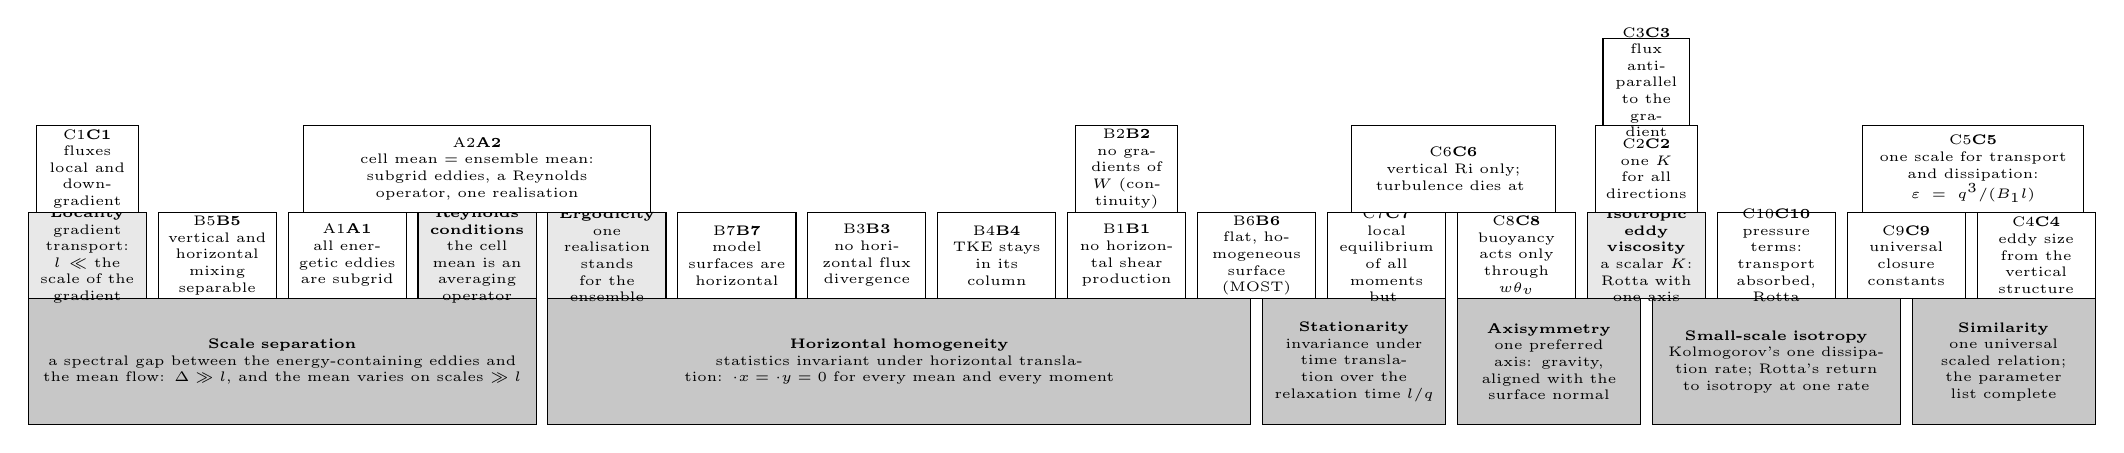
\begin{tikzpicture}[x=1cm, y=1cm,
  ground/.style={draw, line width=0.4pt, fill=black!22},
  hyp/.style={draw, line width=0.4pt, fill=black!9},
  row/.style={draw, line width=0.4pt, fill=white}]
% ---- level 0: the ground (y 0 -- 1.6) ----------------------------------------
\pb{0}{6.45}{0}{1.6}{ground}{\textbf{Scale separation}\\ a spectral gap between the energy-containing eddies and the mean flow: \mbox{$\Delta \gg l$}, and the mean varies on scales \mbox{$\gg l$}}
\pb{6.6}{15.525}{0}{1.6}{ground}{\textbf{Horizontal homogeneity}\\ statistics invariant under horizontal translation: \mbox{$\pd{\avg{\cdot}}{x} = \pd{\avg{\cdot}}{y} = 0$} for every mean and every moment}
\pb{15.675}{18.0}{0}{1.6}{ground}{\textbf{Stationarity}\\ invariance under time translation over the relaxation time $l/q$}
\pb{18.15}{20.475}{0}{1.6}{ground}{\textbf{Axisymmetry}\\ one preferred axis: gravity, aligned with the surface normal}
\pb{20.625}{23.775}{0}{1.6}{ground}{\textbf{Small-scale isotropy}\\ Kolmogorov's one dissipation rate; Rotta's return to isotropy at one rate}
\pb{23.925}{26.25}{0}{1.6}{ground}{\textbf{Similarity}\\ one universal scaled relation; the parameter list complete}
% ---- level 1 (y 1.6 -- 2.7): 16 blocks of 1.5 cm, air gap 0.15 ---------------
\pb{0}{1.5}{1.6}{2.7}{hyp}{\textbf{Locality}\\ gradient transport: $l \ll$ the scale of the gradient}
\pb{1.65}{3.15}{1.6}{2.7}{row}{\pid{B5}\\ vertical and horizontal mixing separable}
\pb{3.3}{4.8}{1.6}{2.7}{row}{\pid{A1}\\ all energetic eddies are subgrid}
\pb{4.95}{6.45}{1.6}{2.7}{hyp}{\textbf{Reynolds conditions}\\ the cell mean is an averaging operator}
\pb{6.6}{8.1}{1.6}{2.7}{hyp}{\textbf{Ergodicity}\\ one realisation stands for the ensemble}
\pb{8.25}{9.75}{1.6}{2.7}{row}{\pid{B7}\\ model surfaces are horizontal}
\pb{9.9}{11.4}{1.6}{2.7}{row}{\pid{B3}\\ no horizontal flux divergence}
\pb{11.55}{13.05}{1.6}{2.7}{row}{\pid{B4}\\ TKE stays in its column}
\pb{13.2}{14.7}{1.6}{2.7}{row}{\pid{B1}\\ no horizontal shear production}
\pb{14.85}{16.35}{1.6}{2.7}{row}{\pid{B6}\\ flat, homogeneous surface (MOST)}
\pb{16.5}{18.0}{1.6}{2.7}{row}{\pid{C7}\\ local equilibrium of all moments but $\qsq$}
\pb{18.15}{19.65}{1.6}{2.7}{row}{\pid{C8}\\ buoyancy acts only through $\avg{w\theta_v}$}
\pb{19.8}{21.3}{1.6}{2.7}{hyp}{\textbf{Isotropic eddy viscosity}\\ a scalar $K$: Rotta with one axis}
\pb{21.45}{22.95}{1.6}{2.7}{row}{\pid{C10}\\ pressure terms: transport absorbed, Rotta}
\pb{23.1}{24.6}{1.6}{2.7}{row}{\pid{C9}\\ universal closure constants}
\pb{24.75}{26.25}{1.6}{2.7}{row}{\pid{C4}\\ eddy size from the vertical structure}
% ---- level 2 (y 2.7 -- 3.8) ---------------------------------------------------
\pb{0.1}{1.4}{2.7}{3.8}{row}{\pid{C1}\\ fluxes local and down-gradient}
\pb{3.5}{7.9}{2.7}{3.8}{row}{\pid{A2}\\ cell mean $=$ ensemble mean: subgrid eddies, a Reynolds operator, one realisation}
\pb{13.3}{14.6}{2.7}{3.8}{row}{\pid{B2}\\ no gradients of $W$ (continuity)}
\pb{16.8}{19.4}{2.7}{3.8}{row}{\pid{C6}\\ vertical Ri only; turbulence dies at $\Rfc$}
\pb{19.9}{21.2}{2.7}{3.8}{row}{\pid{C2}\\ one $K$ for all directions}
\pb{23.3}{26.1}{2.7}{3.8}{row}{\pid{C5}\\ one scale for transport and dissipation: $\varepsilon = q^3/(B_1 l)$}
% ---- level 3 (y 3.8 -- 4.9): the tip -----------------------------------------
\pb{20.0}{21.1}{3.8}{4.9}{row}{\pid{C3}\\ flux anti-parallel to the gradient}
\end{tikzpicture}
\end{center}
\landscapeclose
